\documentclass[a4paper]{article} 
\usepackage{graphicx} 
\usepackage[ngerman]{babel} 
\usepackage[ansinew]{inputenc} 
\usepackage[T1]{fontenc} 
\usepackage{tgpagella} 
\usepackage{geometry} 
\usepackage{color} 
\usepackage{microtype} 
\usepackage{minted}
\usepackage{caption}
\usepackage[headsepline,footsepline]{scrpage2}
\usepackage{textcomp}
\usepackage{pdfpages}
\usepackage{mdframed}



\makeatletter
\renewcommand\minted@pygmentize[2][\jobname.pyg]{
  \def\minted@cmd{pygmentize -l #2 -f latex -F tokenmerge
    \minted@opt{gobble} \minted@opt{texcl} \minted@opt{mathescape}
    \minted@opt{startinline} \minted@opt{funcnamehighlighting}
    \minted@opt{linenos} -P "verboptions=\minted@opt{extra}"
    -O encoding=UTF-8,outencoding=iso-8859-1 -o \jobname.out.pyg #1}
  \immediate\write18{\minted@cmd}
  % For debugging, uncomment:
  %\immediate\typeout{\minted@cmd}
  \ifthenelse{\equal{\minted@opt@bgcolor}{}}
   {}
   {\begin{minted@colorbg}{\minted@opt@bgcolor}}
  \input{\jobname.out.pyg}
  \ifthenelse{\equal{\minted@opt@bgcolor}{}}
   {}
   {\end{minted@colorbg}}
  \DeleteFile{\jobname.out.pyg}}
\makeatother


\title{Dokumentation - 6 Übung}
\author{Roman Lumetsberger}
\date{\today}

\newmintedfile[ccode]{cpp}{
               linenos,
               numbersep=5pt,
               frame=lines,
               framesep=2mm
}

\newmintedfile[javacode]{java}{
               linenos,
               numbersep=5pt,
               frame=lines,
               tabsize=2,
               framesep=2mm,
}
\newmintedfile[csscode]{css}{
               linenos,
               numbersep=5pt,
               frame=lines,
               tabsize=2,
               framesep=2mm,
}
\newmintedfile[sqlcode]{sql}{
               linenos,
               numbersep=5pt,
               frame=lines,
               tabsize=2,
               framesep=2mm,
}
\captionsetup{
  font=footnotesize,
  justification=raggedright,
  singlelinecheck=false
}


\newcommand{\srcDir}{../Beispiel/src/at/lumetsnet/caas/}
\newcommand{\testDir}{../Beispiel/test/at/lumetsnet/caas/test/}

\definecolor{lineColor}{RGB}{151,0,0}
\pagestyle{scrheadings}
\clearscrheadfoot
\begin{document}
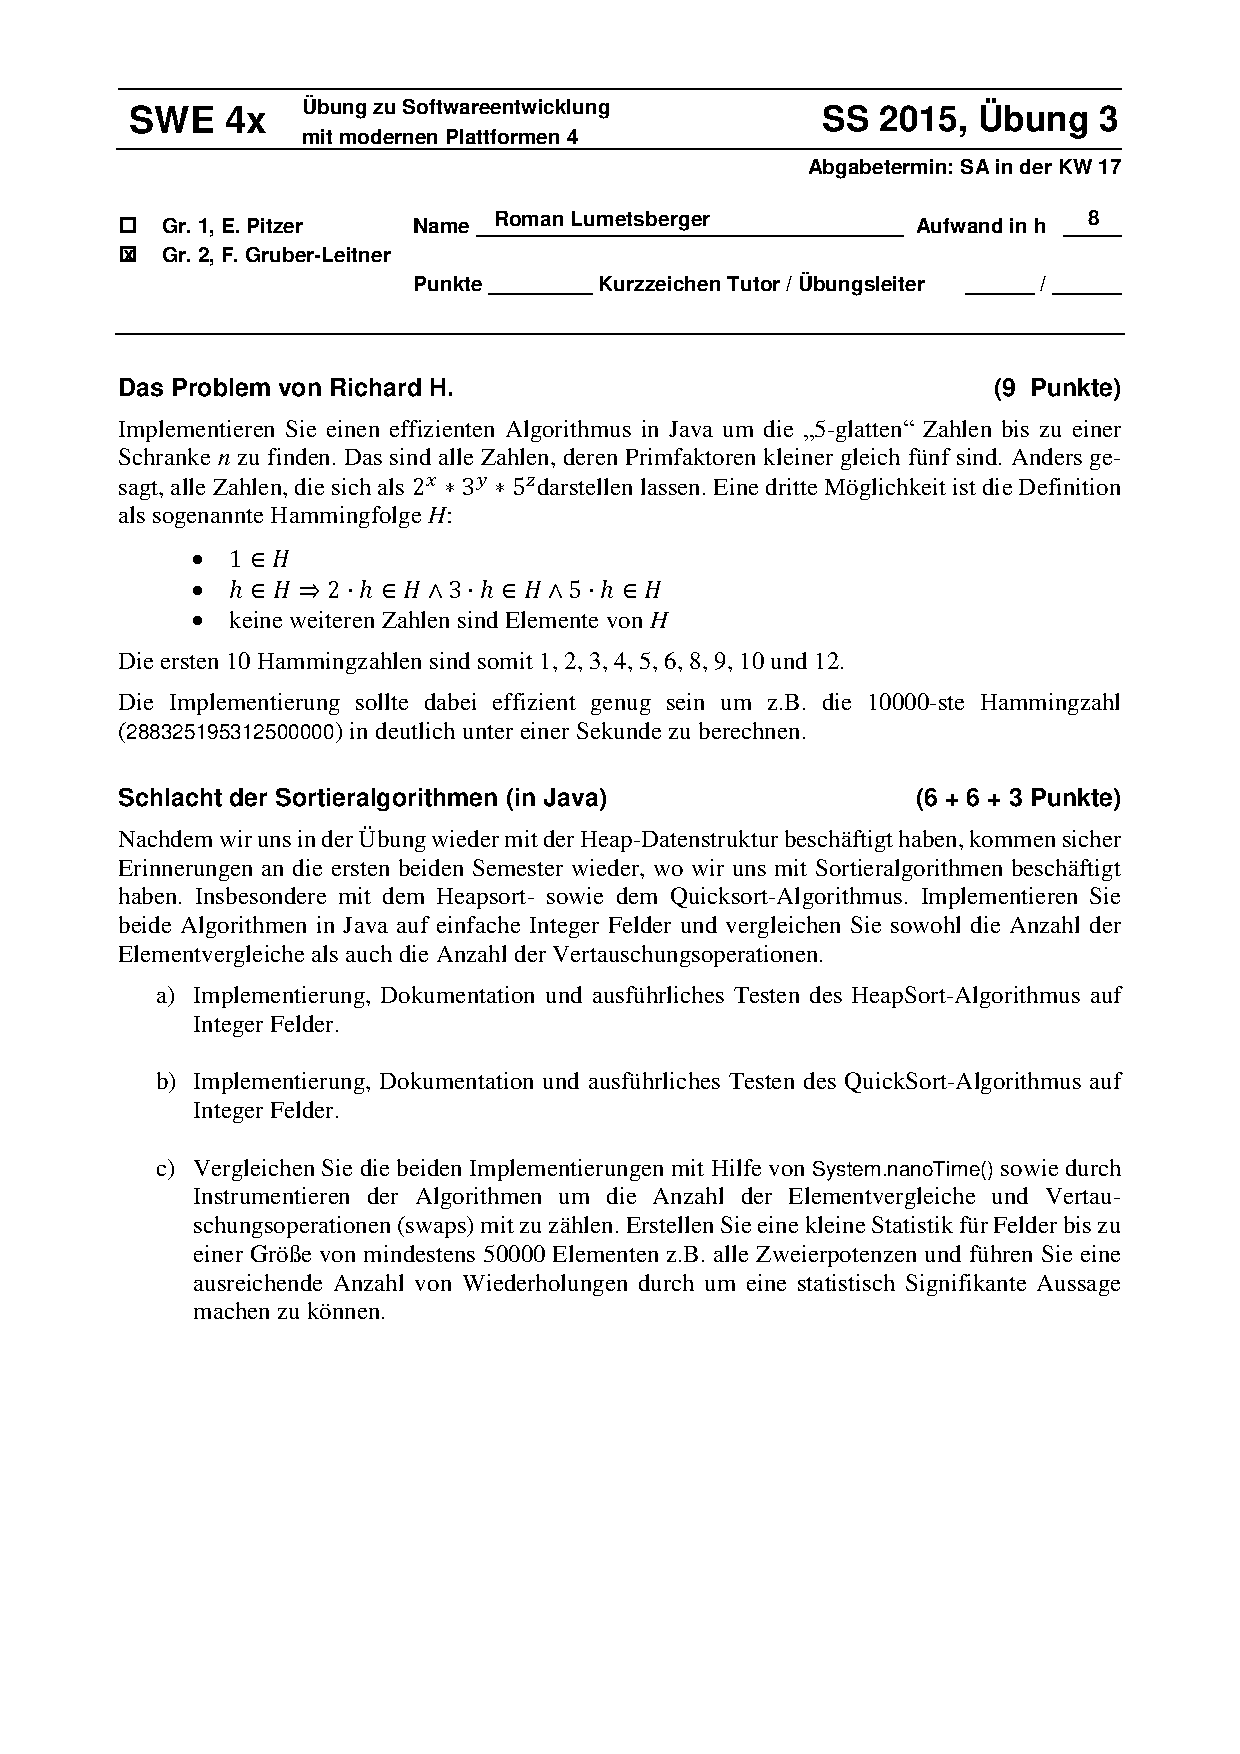
\includepdf[pages=-]{angabe.pdf}

\ihead{SWO3 SS 2015 - �bung 03}
\ifoot{Roman Lumetsberger}
\cfoot{1310307026}
\ofoot{Seite \pagemark}

\section{Das Problem von Richard H. }
\subsection{L�sungsidee}
Die Hammingfolge l�sst sich mit Hilfe der Definition laut Angabe umsetzen. \newline
Dabei wird 1 als erste Hammingzahl in eine Liste eingef�gt. Dann k�nnen die weiteren Zahlen durch multiplizieren mit 2, 3 und 5 hinzugef�gt werden. \newline
Durch Mitf�hren von Index-Variablen wird sichergestellt, dass jede Zahl in der Liste genau einmal mit 2, 3 und 5 multipliziert wird. 
Sobald die angegebene obere Schranke erreicht ist, kann die Schleife beendet werden. \newline

\pagebreak
\subsection{Sourcecode}

\textbf{Hamming.java}
\javacode{../Beispiel/at/lumetsnet/swo/ue3/hamming/Hamming.java}
\textbf{HammingTest.java}
\javacode{../Beispiel/at/lumetsnet/swo/ue3/test/HammingTest.java}

\subsection{Testf�lle}
\begin{center}
\fbox{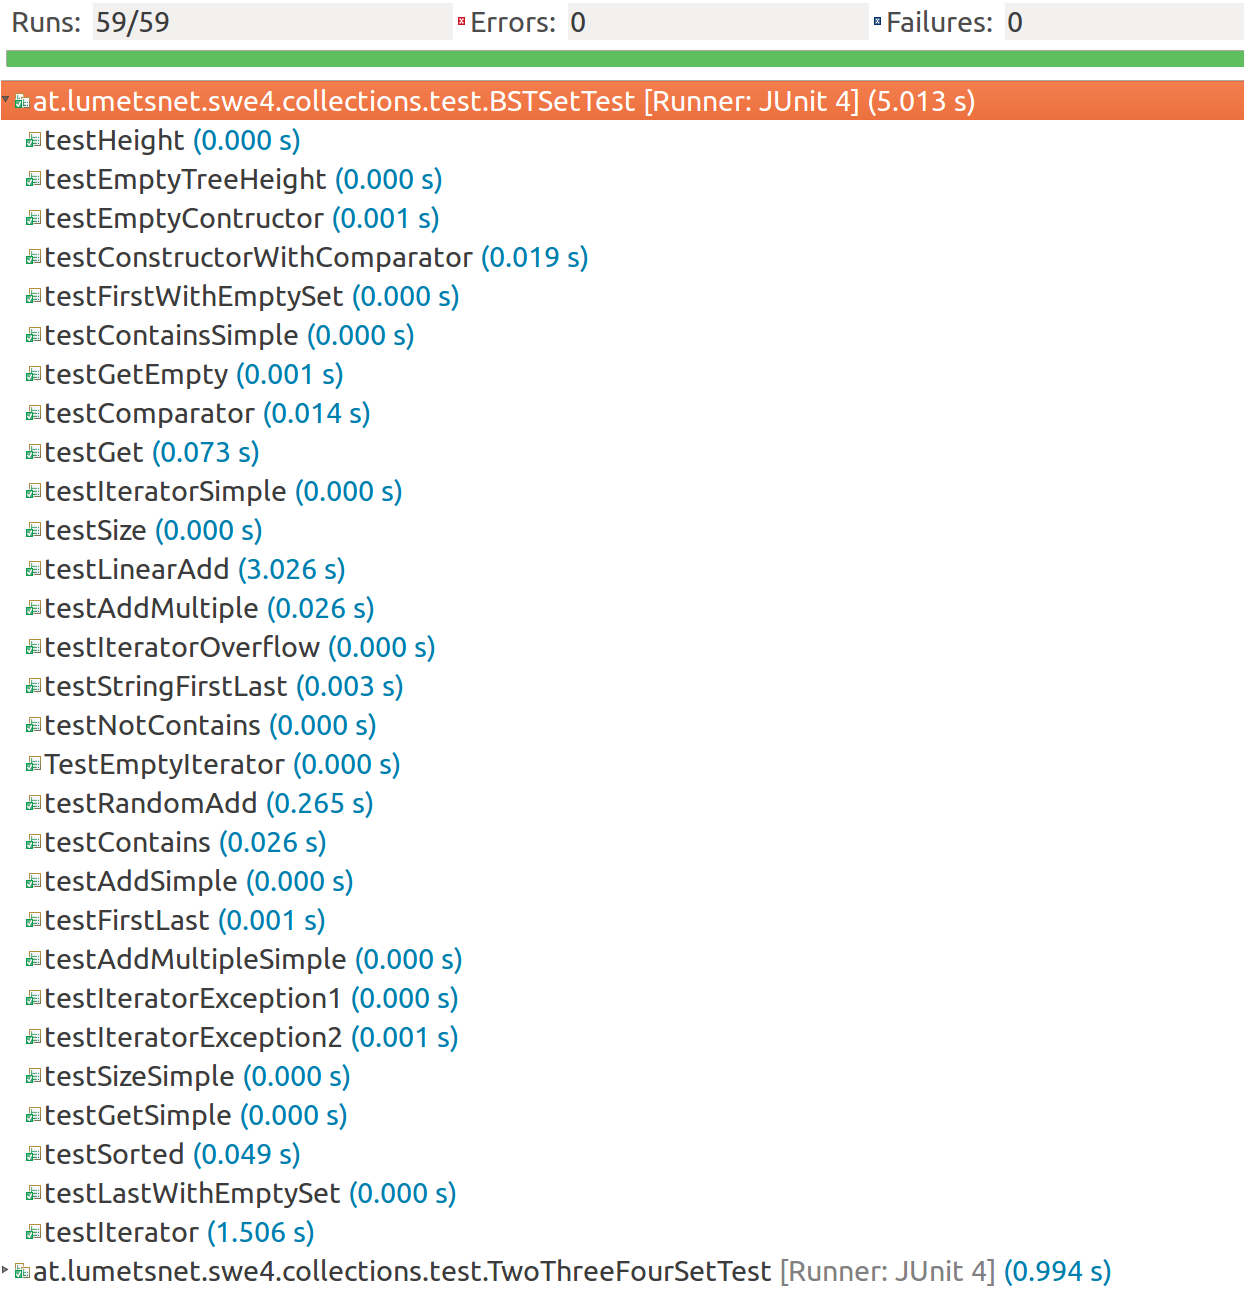
\includegraphics[width=400px]{../Screenshots/1.png}}
\end{center}

\section{Schlacht der Sortieralgorithmen }
\subsection{L�sungsidee}
\subsubsection*{Heapsort}
\begin{itemize}
\item F�r den Heapsort wird zu Beginn das Eingabefeld in einen Heap �bergef�hrt. Damit befindet sich das gr��te Element an erster Stelle.
\item Dieses wird dann mit dem letzten Element vertauscht und die Gr��e um 1 verringert.
\item Danach wird wieder sichergestellt, dass es sich um einen Heap handelt.
\item Damit ist das n�chst gr��ere Element an erster Stelle, welches wieder vertauscht wird.
\item Dies wird dann solange wiederholt bis die Heapgr��e gleich 1 ist.
\end{itemize}

Dann hat man ein aufsteigend sortiertes Feld.

\subsubsection*{Quicksort}
Beim Quicksort wird die Menge in Teillisten getrennt und in sich sortiert. Die Trennung erfolgt durch ein Pivot Element. 
\begin{itemize}
\item In der linken Liste sind jene Elemente, die kleiner als das Pivot Element sind.
\item In der rechten Liste sind jene Elemente, die gr��er als das Pivot Element sind.
\end{itemize}

\subsubsection*{Statistik}
Um die Statistik erstellen zu k�nnen, wird eine eigene Klasse \textit{InstrumentationData} erstellt, die die ben�tigten Daten aufnehmen kann.\newline
Weiters m�ssen die Algorithmen erweitert werden, damit sie die Daten zur Verf�gung stellen. \newline
Durch die neue Basisklasse \textit{Sorter} wird die Instrumentierung abstrahiert.\newline
\textbf{Die Statistik wird in den Testf�llen generiert.}
\pagebreak


\subsection{Sourcecode}
\textbf{HeapSort.java}
\javacode{../Beispiel/at/lumetsnet/swo/ue3/sort/HeapSort.java}
\textbf{QuickSort.java}
\javacode{../Beispiel/at/lumetsnet/swo/ue3/sort/QuickSort.java}
\textbf{InstrumentationData.java}
\javacode{../Beispiel/at/lumetsnet/swo/ue3/sort/InstrumentationData.java}
\textbf{Sorter.java}
\javacode{../Beispiel/at/lumetsnet/swo/ue3/sort/Sorter.java}
\textbf{SortTest.java}
\javacode{../Beispiel/at/lumetsnet/swo/ue3/test/SortTest.java}
\textbf{Main.java}
\javacode{../Beispiel/at/lumetsnet/swo/ue3/test/Main.java}

\subsection{Testf�lle}
\begin{center}
\fbox{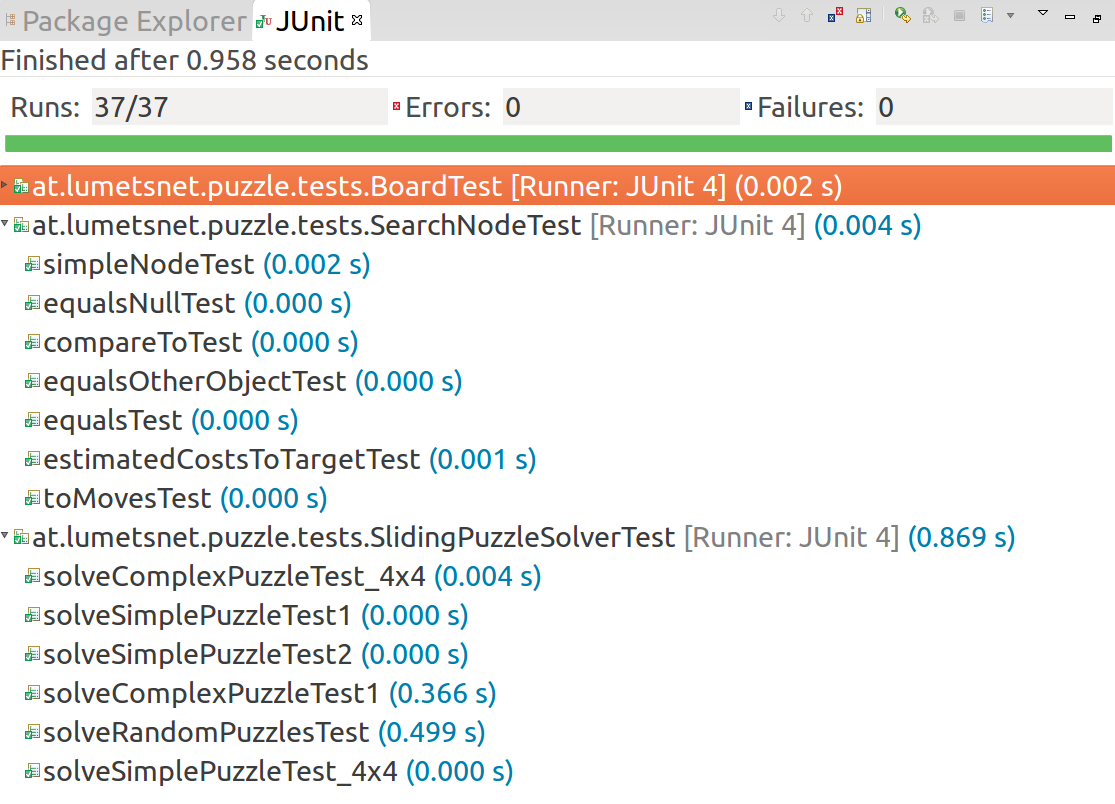
\includegraphics[width=400px]{../Screenshots/2.png}}
\fbox{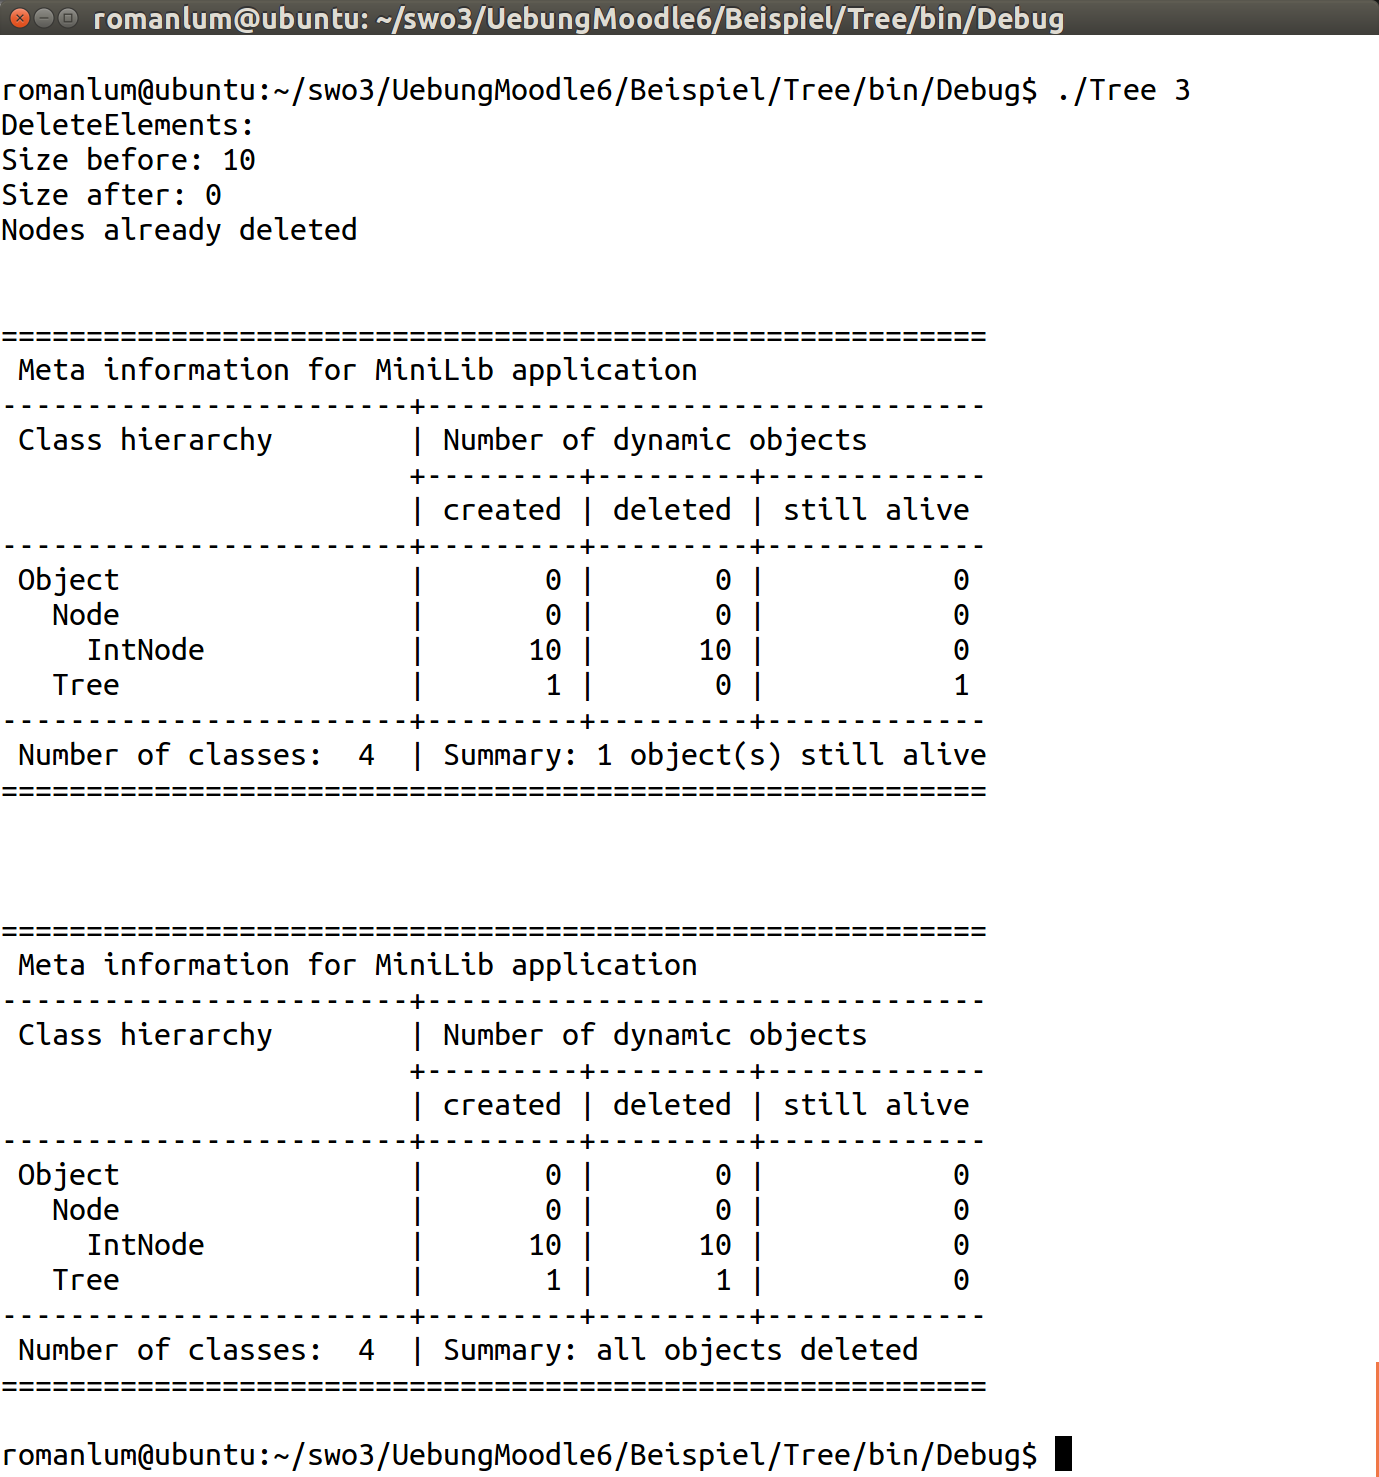
\includegraphics[width=400px]{../Screenshots/3.png}}
\fbox{
\includegraphics[width=400px]{../Screenshots/4.png}}
\fbox{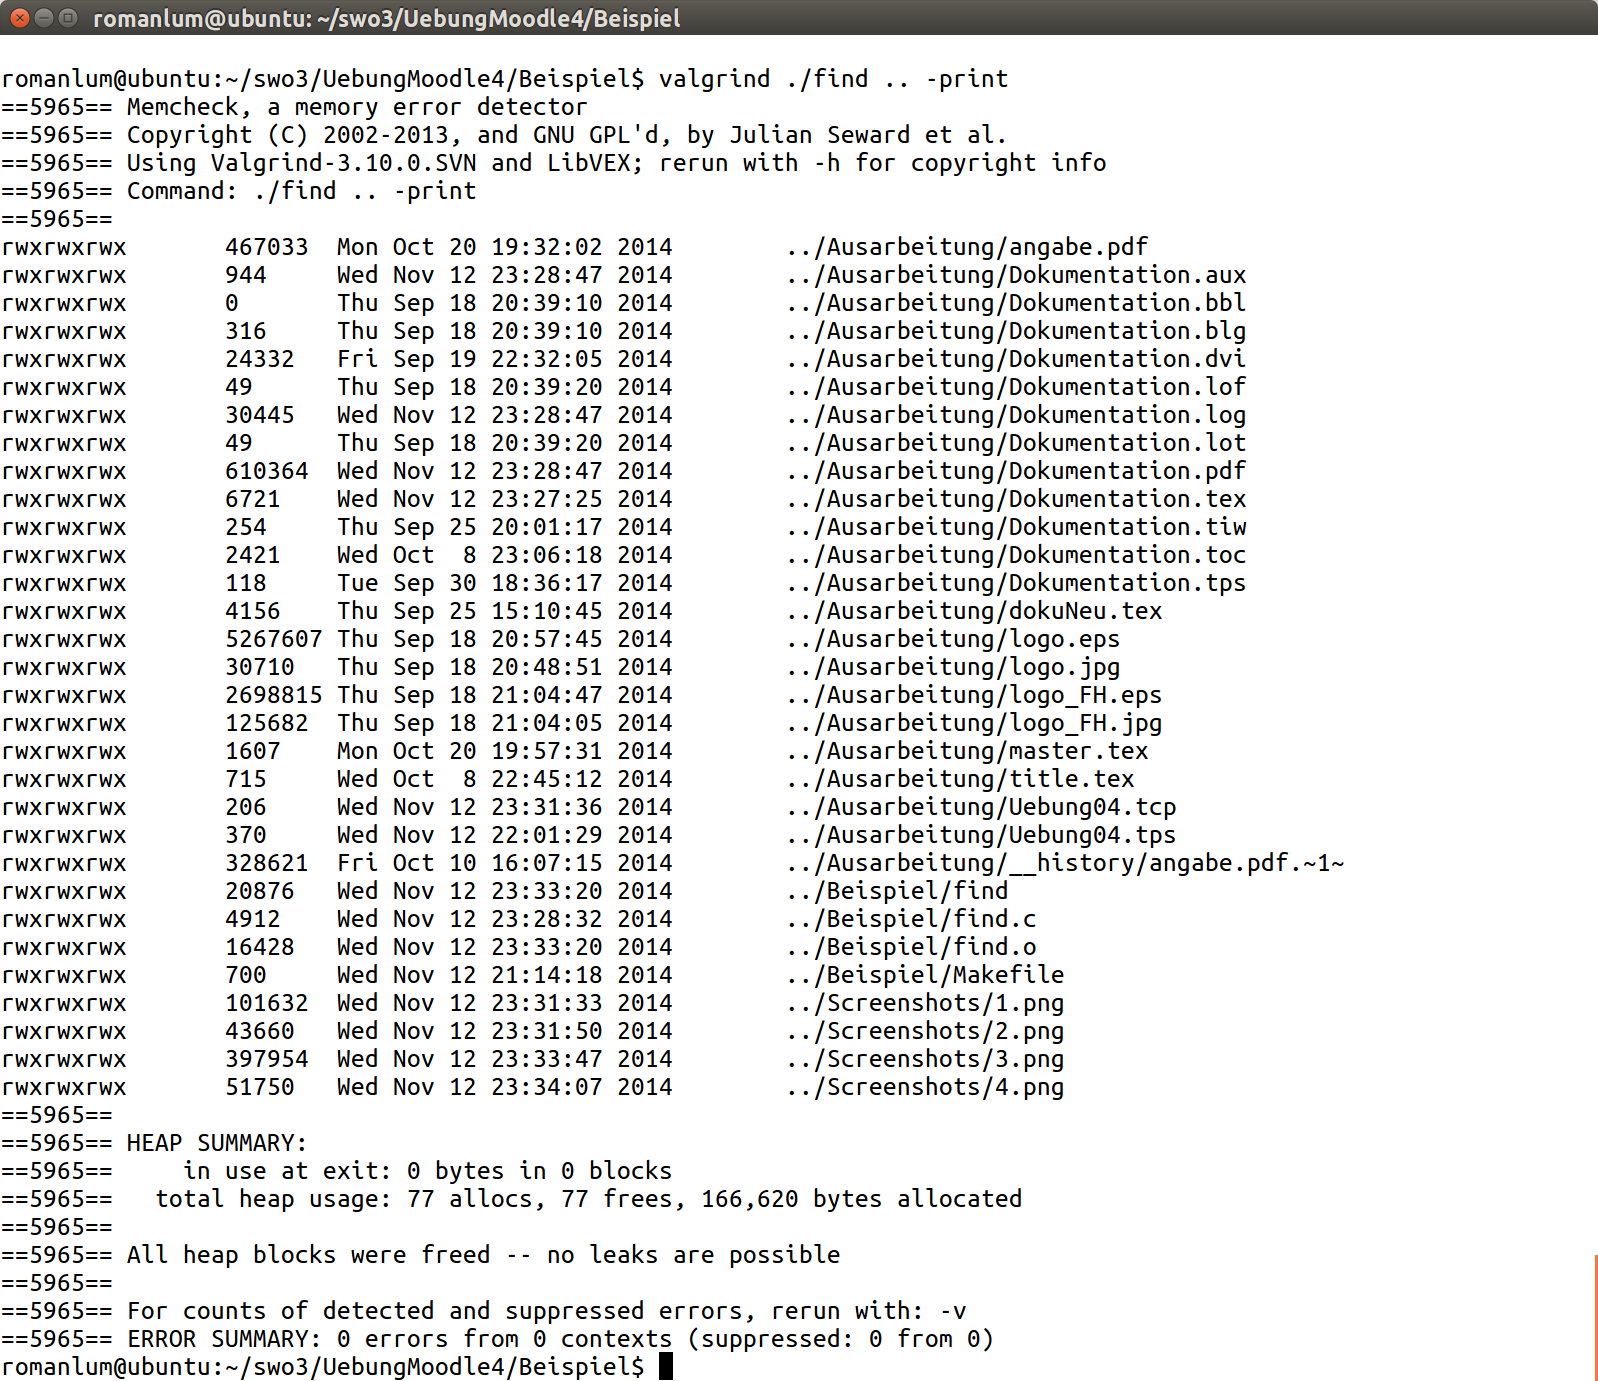
\includegraphics[width=400px]{../Screenshots/5.png}}
\end{center}


\end{document}